\documentclass{xStandalone}

\begin{document}
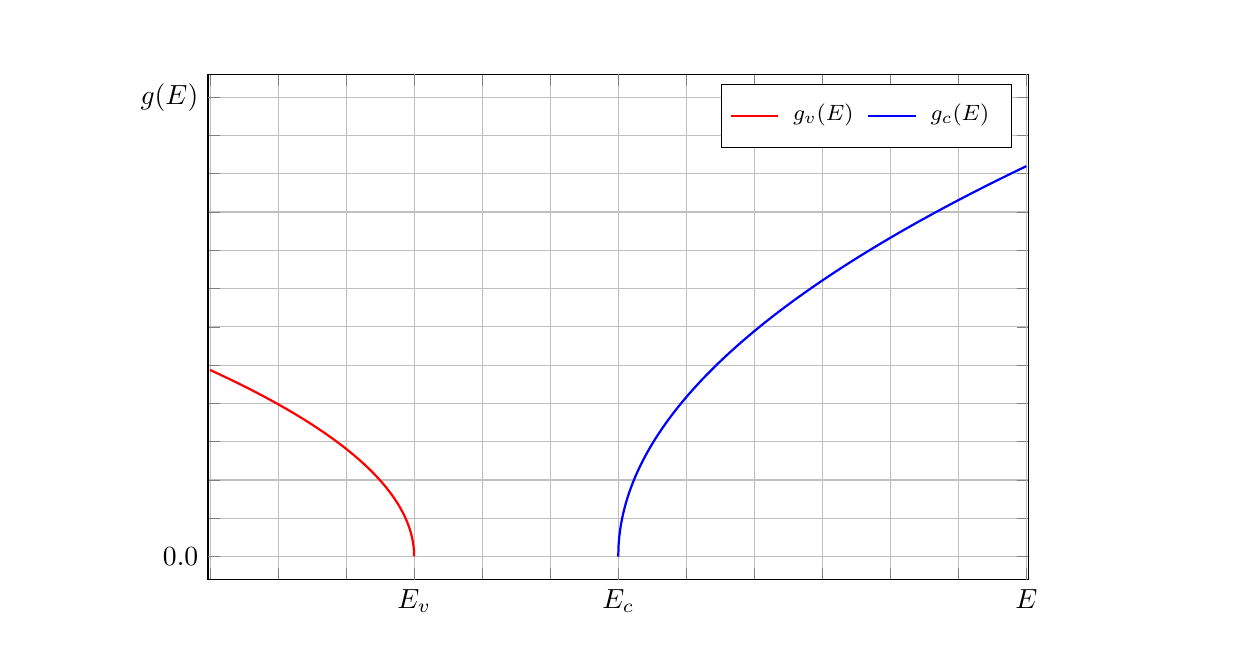
\begin{tikzpicture}

\clip (-7.5,-4) rectangle (7.5,3.8);

\pgfplotsset{every axis legend/.append style=
{nodes={inner sep=5pt,text depth=0.25em}}}
    
\begin{axis}[
ymin=-0.06,ymax=1.26,
xmin=-0.03,xmax=12.03,
anchor=center,
grid,
legend style={font=\footnotesize},
legend entries={
    $g_\text{v}(E)$\\$g_\text{c}(E)$\\},
legend cell align=right,
legend columns=2,
width=12cm,
height=8cm,
xtick={0,1,...,12},
xticklabels={},
ytick={0,0.1,...,1.2},
yticklabels={},
extra x ticks={3,6,12},
extra x tick labels={$E_\text{v}$,$E_\text{c}$,$E$},
extra y ticks={0,1.2},
extra y tick labels={$0.0$\\$g(E)$\\},
mark size=1
]

\addplot[domain=0:3,samples=1000,thick,red,line legend] 
{0.4*(0.59)^(2/3)*(3-x)^(1/2)};
\addplot[domain=6:12,samples=1000,thick,blue,line legend] 
{0.4*(1.062)^(2/3)*(x-6)^(1/2)};


% \addplot[white] coordinates{(4,0.5)} node[point] {};
% \addplot[white] coordinates{(4,1.0)} node[point] {};

\end{axis}

\end{tikzpicture}
\end{document}